\chapter{Architettura}
\label{sec:architettura}

\begin{figure}
    \centering
    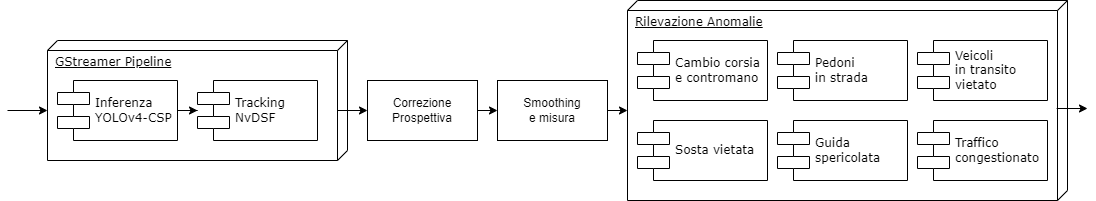
\includegraphics[width=\textwidth]{images/arch.png}
    \caption{Architettura del sistema}
\end{figure}

Il sistema ottiene e decodifica lo stream video proveniente dalla camera sfruttando la libreria \emph{GStreamer}\cite{arch:gstreamer}, che permette di creare una pipeline di acquisizione video in grado di supportare svariati protocolli e formati. 
All'interno di questa pipeline sono inoltre installati due moduli forniti dall'\emph{SDK Nvidia Deepstream}\cite{arch:deepstream}:
\begin{itemize}
    \item Il modulo di inferenza, che con la configurazione fornita da M.Luciano \cite{marcosluciano} utilizza \emph{Scaled-YOLOv4}\cite{yolocsp} per rilevare le entità presenti nella scena.
    \item Il modulo di tracking \emph{NvDCF}\cite{nvdcf}, che identifica le entità rilevate dall'inferenza.
\end{itemize}

I dati ottenuti vengono poi inviati dalla pipeline di acquisizione al modulo di correzione della prospettiva, che utilizzando le tecniche descritte nel capitolo \ref{sec:posizione} calcola la posizione delle entità nello spazio reale.

Il modulo di smoothing e misura confronta i dati, e in particolare la posizione, delle entità con quelli ottenuti in passato e, utilizzando l'algoritmo descritto nel capitolo \ref{sec:velocita}, fornisce misure più affidabili per posizione e velocità delle entità.

Questi dati arrivano quindi al modulo di rilevazione anomalie, che identifica le situazioni di rischio e le comunica a sistemi esterni.
Il sistema di rilevazione anomalie è composto da vari sotto-moduli, ognuno dei quali implementa euristiche per la rilevazione di una singola tipologia di anomalia. Questi sottomoduli sono:
\begin{itemize}
    \item Cambio corsia e contromano, che rileva veicoli in contromano o veicoli che oltrepassano una striscia continua
    \item Sosta vietata, che rileva veicoli che restano fermi per lunghi tempi in luoghi dove non è permessa la sosta
    \item Pedoni in strada, che rileva i pedoni che attraversano la strada dove non permesso
    \item Guida spericolata, che rileva i veicoli che esibiscono comportamenti rischiosi, come ad esempio un alta velocità
    \item Veicoli in transito vietato, che rileva i veicoli in transito in zone dove questo non è permesso, come marciapiedi o isole di traffico
    \item Traffico congestionato, che rileva quando è presente un alto numero di veicoli e il flusso del traffico è da questo limitato
\end{itemize}

Il sistema è implementato sul dispositivo \emph{Nvidia Jetson Xaxier}\cite{arch:jetson} ed è sviluppato su \emph{Ubuntu 18.04}\cite{arch:ubuntu}.
Il linguaggio di sviluppo è \emph{Python 3.6}\cite{arch:python}.
Per le operazioni di algebra lineare sono state utilizzate le librerie \emph{Numpy}\cite{arch:numpy} e \emph{SciPy}\cite{arch:scipy}.
La segnalazione delle anomalie è effettuata utilizzando la libreria \emph{Requests} \cite{arch:requests}.
L'annotazione del video con le informazioni generate dal sistema e il suo encoding è realizzato con la libreria \emph{OpenCV} \cite{opencv}.
